%------------------------------------------------------------------------------
% No implementation, software engineering details, or project management
%------------------------------------------------------------------------------

%------------------------------------------------------------------------------

\begin{subsection}{The Elevator Pitch}
  Advances in technology have revolutionised other industries and parts of agriculture, bringing with it radically improved methods and cost efficiencies. However, the method used to identify and mark cattle has practically remained archaic.

  Globally, and particularly in developing countries, cattle are revered. They often represent a high percentage of a farmer's livelihood and wealth. It is in these countries where generally, cattle are the least protected from theft.

  CowHub provides access to a database of cattle which can be used to identify cattle without the need for physical deformation. In doing so, any cattle that has not been tampered with can be identified as belonging to it's owner deterministically and with near certain reliability.
\end{subsection}

%------------------------------------------------------------------------------

\begin{subsection}{Project Description}
  This project will focus on providing a technology-based answer to the problem aformentioned. It will consist in developing a user-friendly platform that uses a scalable and centralised cattle management and identification system. The three key objectives for this project are the following:

  \begin{itemize}
  	\item Offer a \textbf{harmless, physically non-destructive alternative} to current methods used to identify cattle
  	\item Provide a service that \textbf{allows the identification of cattle}
  	\item Collect data on cattle from farmers to be able to \textbf{build and use a widespread catalogue of information regarding cattle and their movements}
  \end{itemize}

\end{subsection}

%------------------------------------------------------------------------------

\begin{subsection}{What is the need for the project?}
  The process of marking cattle can be incredibly painful, regardless of the age of the cattle and is a point of controversy for animal rights activists. Clearly, being subject to this pain or witnessing its offspring being subject to this the pain can be traumatic for a cow. Members of the public feel so strongly about the issue that they have protested by branding themselves in public, much to the disgust of onlookers~\cite{theguardian1}.

  Whilst branding itself is no longer carried out in the United Kingdom, current methods, including piercing a cattle's ears, are still in use today and are without animal-friendly competition currently.

  \begin{figure}[H]
  	\centering
    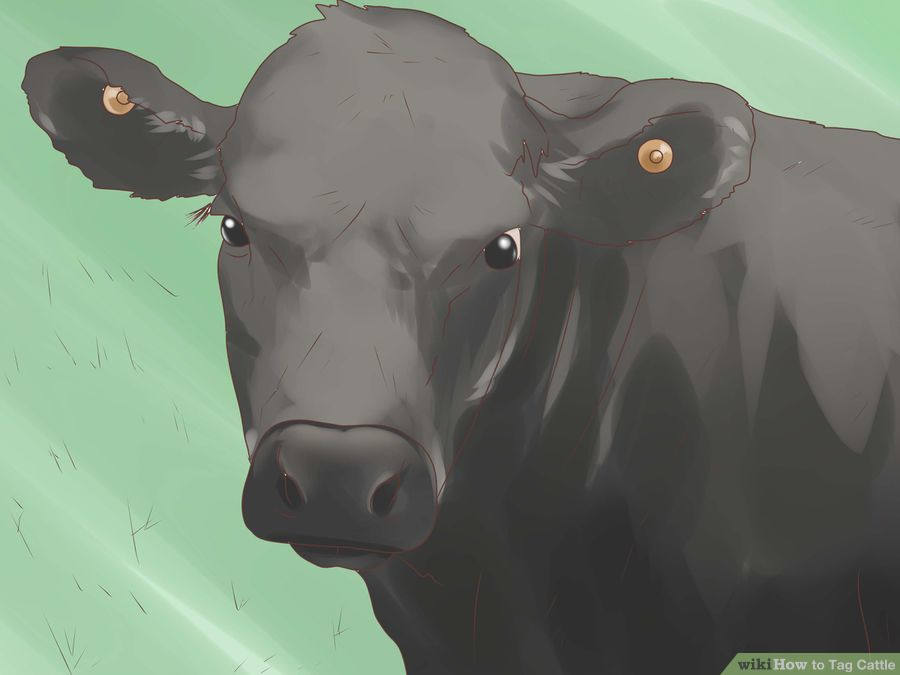
\includegraphics[width=0.5\textwidth]{images/cattle-with-ear-tag.jpg}
  	\caption[Cattle ear tagging]{
      Illustration of a cattle's head, demonstrating the position and rough size of cattle tags from the front. \cite{wikihow1}
  	}
  \end{figure}

  CowHub not only provides a user friendly platform to easily register and manage the information of a cattle. But, it also offers a non-intrusive solution to cattle recognition and by doing so alleviates all tagging associated pain with the current system.

\end{subsection}
